\chapter{Musical instruments}

`Is it a real saw?' Many people comment on the saw I keep on a shelf in my office. And, yes, it is a real saw, although it is branded as a `musical saw' and sold under the name Sandviken Stradivarius (Figure~\ref{fig:sandviken}). However, it does not differ much from the ordinary, well-used, crosscut hand saw I use for cutting up wood for the fireplace at home. The main difference is that the musical saw has a logo of a saw musician on the side. Does that make it into a musical instrument? No, if we think that saws were originally designed for cutting wood. However, the Sandviken Stradivarius is designed, manufactured, and branded as a musical instrument. I occasionally play it in my office, so my exemplar is used for musicking. The same is true for my other saw. I have played on that one, too, even though it was not made for performance. My two saws were manufactured with different intentions, but if one disregards the logo, they look alike. Both can produce sound and have music-making potential. They can also both be used to cut wood, although I am pretty sure that I would not reach for the Stradivarius first.

\begin{figure}[tp]
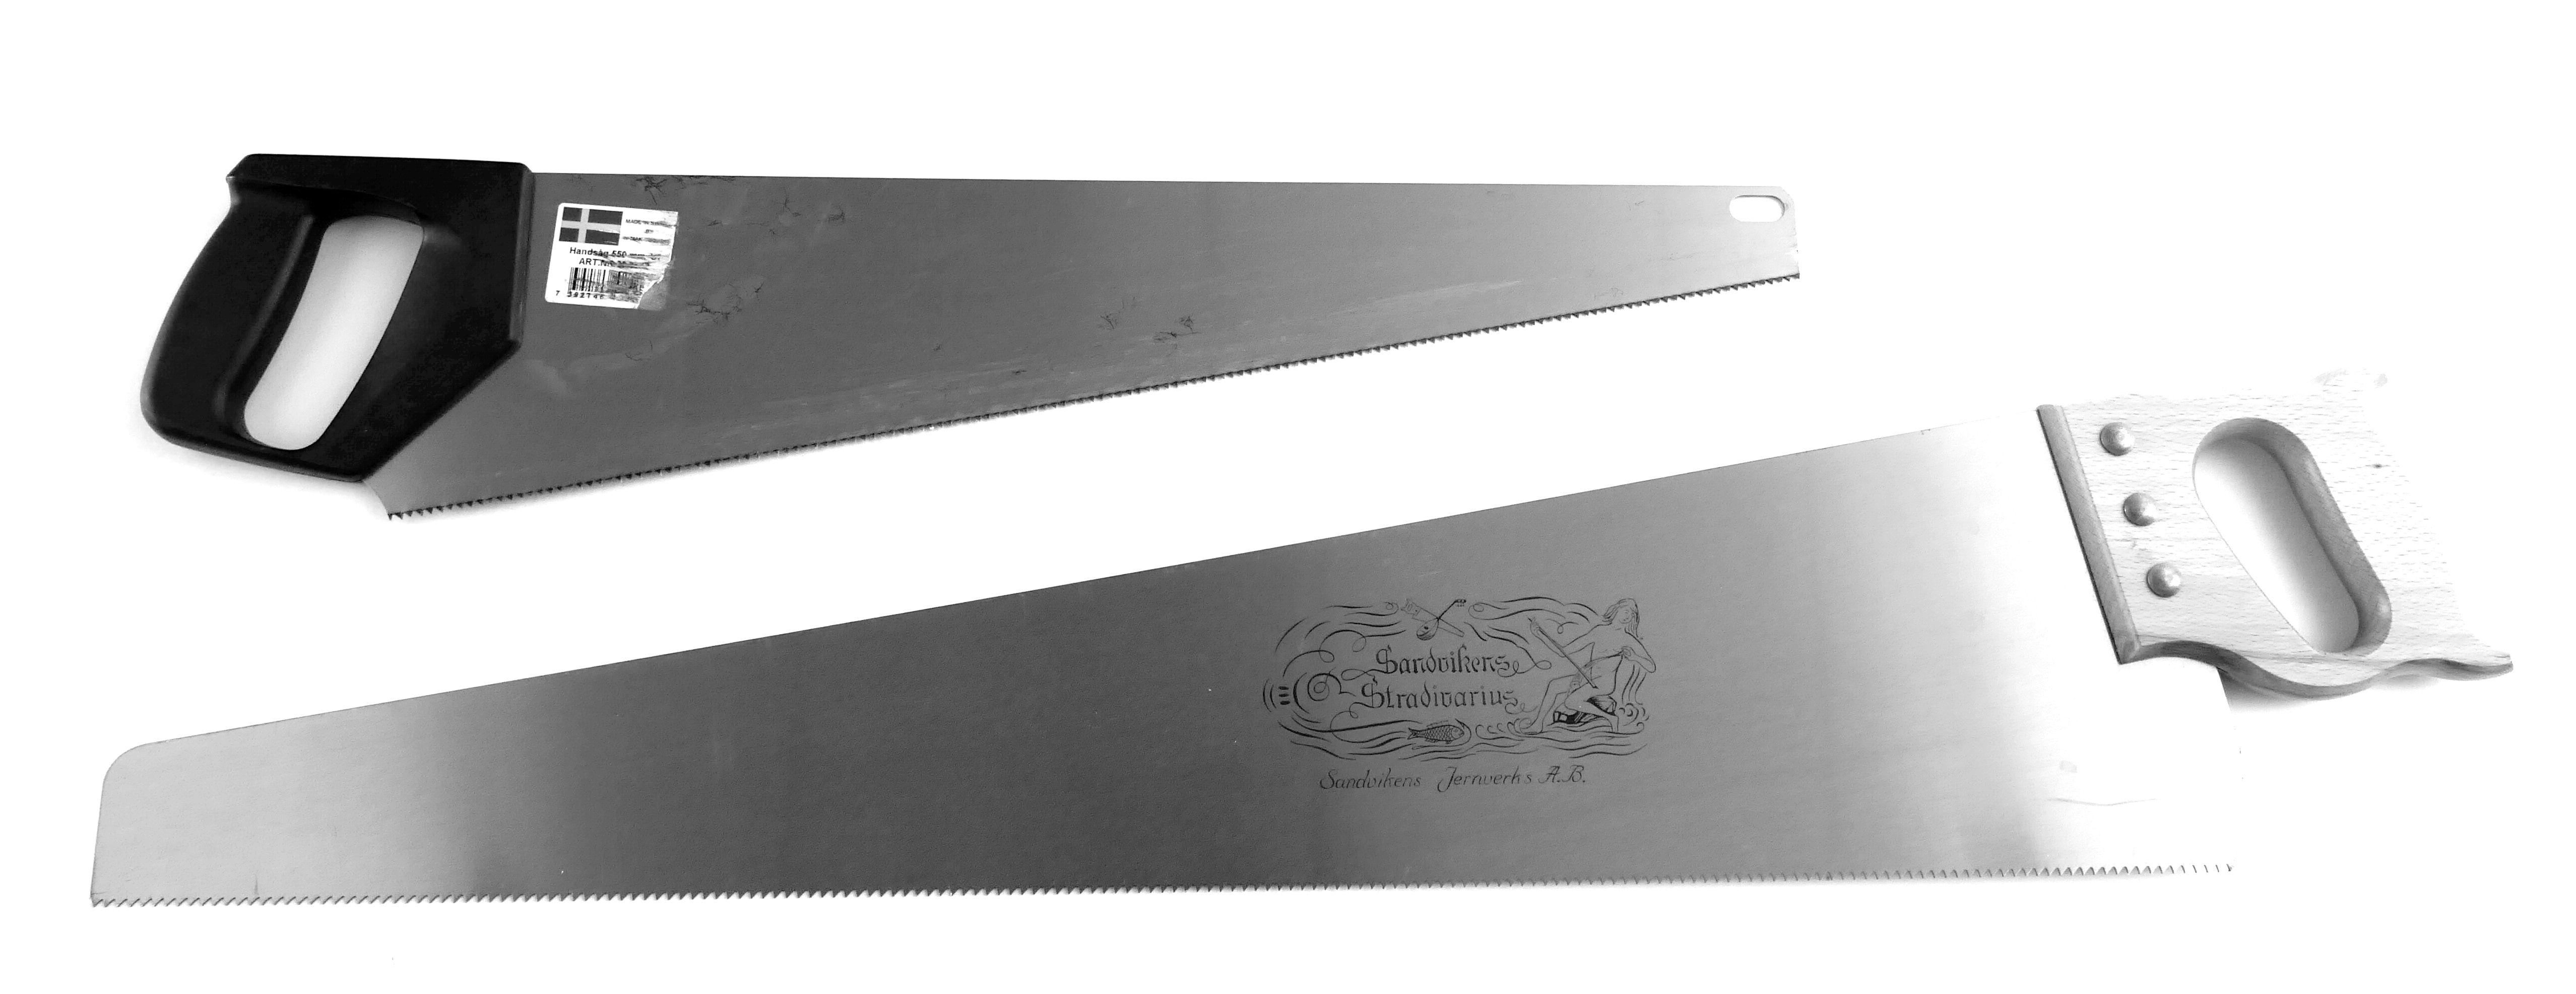
\includegraphics[width=\columnwidth]{figures/15-saw6.jpg}
\caption{The Sandviken Stradivarius (bottom) is a saw made for music performance. How does it differ from an ordinary crosscut hand saw (top)?}
\label{fig:sandviken}
\end{figure}



\section{What is a musical instrument?}

An oboe is a musical instrument. So are charangos, clarinets, and castanets. These are all physical devices made with the intent of performing music. What about a spoon, a bucket, or a chair? Are they also musical instruments? From a design perspective, they are not since they were not originally made for musical activities. However, from a user's perspective, a spoon may be turned into a musical instrument if used in a performance. I find these dichotomies between design intentions and usage fascinating.

For a long time, music research has focused on works \citep{goehr_imaginary_1992} and the composition and performance of such works \citep{johnson_musical_1997}. The works have traditionally been studied as fixed products, either in the form of scores (compositions), recordings (of performances), or productions (of pieces/tunes). Much less attention has been devoted to the role of musical instruments, how they are made, how they look, how they feel, and how they sound. This is the case even though \emph{organology}---the academic study of instruments---has been a well-established discipline for more than a century. Even so, when I ask incoming bachelor's students about what they know about organology, they stare at me with blank eyes.

`Everyone' agrees that instruments are essential for musicking. Still, instruments receive relatively attention in musicological discourse. There are some notable exceptions, including investigations into the `social life' of instruments \citep{bates_social_2012}, thoughts on instruments as `creative prostheses' \citep{de_souza_music_2017}, and reflections on 21st century instruments \citep{bovermann_musical_2017}. Yet, often the importance of instruments is forgotten. In my opinion, a better understanding of musical instruments is key to understanding how musicking at large is in transition. From here on, we will shift our attention to musical instruments and look at their construction and function in both acoustic and electro-acoustic musicking.


\section{Instrument identity}

The musical saw represents a borderline case between design intention, usage, and cultural connotation. This example also shows that defining an instrument is not as easy as one may think. As we shall see later, it becomes more complicated when considering electro-acoustic instruments. But is this a problem? Does it matter how we define a musical instrument? \citet{kvifte_what_2008} cautions against trying to define what an instrument should be, worrying that:

\begin{quotation}
If a traditional and relatively precise definition of ‘instrument’ excludes large areas of contemporary musical practice from our field of study, we might be better off with less precise alternatives.
\end{quotation}

In my experience, instrument definitions are more important than we like to acknowledge. For example, in higher music education, the norm is still to play `an instrument.' I am constantly reminded about this when I participate in our department's welcome lunch for new music students each fall semester. Listening to the students introducing themselves is fascinating. They usually start by stating their name and the school they attended before coming to university. Almost without exception, the third thing they mention is what instrument they play. Their instrument defines who they are as aspiring professionals.
Some students say they play `the piano.' However, this often leads to follow-up questions about genre. Playing `classical piano' or `jazz piano' is not the same. Their sound-maker---the physical piano---may be the same, but their use of it differs. It helps to add the genre to the naming of their instrument to explain their musical identity. As such, the genre becomes a sub-category of the naming of the physical instrument. This may not be as strange as it sounds. In many cases, the performance technique differs between genres. If you say that you play `contemporary piano,' one may think that you spend a considerable amount of time fiddling inside the piano, touching the strings, adding objects, or developing extended techniques. This is different from playing `classical piano.'

For piano, it is common to add the genre as a prefix to the instrument's name. There are also examples of how the naming of the instrument itself is dependent on the genre. \citet{kvifte_instruments_1989} discusses the distinction between the instrument(s) `fiddle' and `violin.' In most cases, these terms refer to the same type of instrument. An exception is the Norwegian Hardanger fiddle, with four resonating strings below the normal strings, although this instrument would probably be called `Hardanger fiddle' and not only `fiddle.' When it comes to normal fiddles and violins, they are the same physical instrument. However, they are often played differently. Most violinists would rest their instrument towards the chin, while fiddlers may rest it on their arm. Some Indian classical musicians sit cross-legged on the floor resting the violin's head at the sole of their feet \citep{magnusson_migration_2021}. Not only do the genres lead to different naming of the instruments, but also the naming of the performers. A `fiddler' is not the same as a `violinist.' This is not just a question about terminology; it also defines a musician's training and career.

There are also examples of how the naming of an instrument may cover different types of physical instruments, such as when people say: `I play keys.' In most cases, this would indicate that the person plays one or more types of keyboard-based instruments. This often includes both acoustic piano and various kinds of analog and digital keyboards. Most likely, `keys' would also indicate that the person plays popular music or jazz. I have still to come across a classical performer stating that they play `keys.'

What instrument you play matters. After all, professional identities are built around instruments. Being `a fiddler,' `a pianist,' or `a DJ' defines what you do and who you are in the music world. Conservatories and universities recruit students based on instrument type, and so do most traditional orchestras (`Searching for a violinist...') and bands (`Looking for a bass player...'). Also, many non-musicians have a clear idea about what the different terms mean.
When I tell people that I work with music, people always ask about my instrument. It is difficult to answer such a question. I could be honest and say that I design, build, and play various body-based electro-acoustic instruments. However, if I do not want to get into lengthy explanations, I say that `I play the piano.' That is a straightforward answer and it is not entirely false given that the piano is my `mother instrument,' so to speak. The normal follow-up reply, then, is something like: `I used to play the piano as a child.' This is the case even though the person may not have touched the instrument in decades. Still, a person's instrumental childhood experience is something they carry on as part of their identity.

As electronics have become more popular, it is nowadays quite common to hear students say, `I play laptop' or `my DAW is my instrument.' I find such statements interesting because they indicate the shift that this book is all about. We will return to such cases later. In the rest of this chapter, we will primarily focus on traditional acoustic instruments.


\section{Instrument definitions}

It is clear that the naming of instruments matters, but we have not yet come closer to a proper definition of an instrument. As the discussion so far has revealed, coming up with a proper definition is not easy. The Grove Music dictionary ultimately resigns in their article on `instrument' \citep{brown_instrument_2001}:

\begin{quotation}
Like many other musical terms, however, the word meant various things at various times, and it was not always used consistently.
\end{quotation}

Their entry on `musical instrument' is better at explaining the historical notion of instruments and their limitations \citep{libin_musical_2018}:

\begin{quotation}
Conventionally the term refers to implements specially designed for producing sound, but this definition is inadequate because unaltered natural objects as well as utensils meant for other tasks (nowadays including electronic communication devices) have been put to musical use since prehistoric times.
\end{quotation}

This resonates well with my thinking, although the terms implements and utensils do not sound particularly musical. The final definition of an instrument is more focused, though, and is the one that I will continue to use in this book \citep{libin_musical_2018}:

\begin{quotation}
Vehicle for exploring and expressing musical ideas and feelings through sound.
\end{quotation}

There are several reasons why I like this instrument definition. One is that \emph{sound} is at the core of the definition. On a side note here, one could always question whether you need sound to call something music. For example, there have been several experiments with creating \emph{visual music} \citep{evans_foundations_2005,mcdonnell_finding_2020}. We will leave such borderline cases aside for now, though, and assume that sound---including the sound of silence \citep{cage_silence_1961}---plays a significant role in musicking at large.

I also like Libin's use of vehicle instead of, say, tool  or device in the definition. This opens for including the human body and the human voice as instruments. The definition further opens for both exploration and expression, indicating an active and embodied thinking about musicking. The same can be said about including both ideas and feelings, acknowledging that musick covers both structures and emotions.

In a linguistic study of musical instrumentality, \citet{cance_musical_2017} concludes that the term instrument refers to a device and its interaction with the users. I will use such an application-focused definition of musical instruments as a point of departure. Generally speaking, we may say that an instrument can be a mediator between action and sound \citep{bielawski_instrumentalmusik_1979,kvifte_instruments_1989}, as sketched in Figure~\ref{fig:instrument1}. An instrument can be a physical device, but also the human body, a virtual device, or even just an imaginary idea. We will get back to all of these later.

\begin{figure}[tbp]
	\centerline{
		  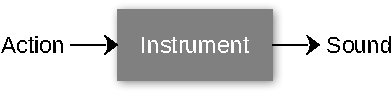
\includegraphics[width=0.5\textwidth]{figures/16-action-sound-crop.pdf}
			\caption{A musical instrument can be seen as a mediator between action and sound.}
			\label{fig:instrument1}
}
\end{figure}

When I emphasize sound in the definition of a musical instrument, this does not necessarily mean \emph{musical} sound. In the same way that a spoon may be used to create musical sound, a musical instrument may be used to make non-musical sound. Accidentally dropping a guitar on the floor will produce sound, but it would usually not be considered musical. With our current definition of an instrument, any device, from spoon to computer, may be considered a musical instrument if used to make music. As we shall see later, the musical content and context may even be integrated into the instrument itself. However, before exploring such complexities, we will rewind a little and consider some traditional ways of thinking about instruments.


\section{The Hornbostel Sachs system}\label{sect:organology}

Up until the late 19th century, instruments were usually sorted into three categories: strings, wind, and percussion \citep{lee_hornbostel-sachs_2019}. Based on work at the instrument museum in Brussels, \citet{mahillon_catalogue_1880} proposed a division into four types, based on the sound production of the instruments: autophones, membranes, wind, and chords. This was further developed into what has become the most well-known musical instrument categorization, often known as the \emph{Hornbostel Sachs} system. This system was first introduced in the book \emph{Systematik der Musikinstrumente} \citep{von_hornbostel_systematik_1914,von_hornbostel_classification_1961}. Building on the work by Mahillon, it classifies musical instruments based on their sound-producing elements:

\begin{description}
  \item[Idiophones:] the material itself generates the sound (e.g. xylophone)
  \item[Membranophones:] a vibrating membrane generates the sound (e.g. drum, kazoo)
  \item[Chordophones:] a moving string generates the sound (e.g. violin, piano)
  \item[Aerophones:] a vibrating air-column generates the sound (e.g. oboe, clarinet, saxophone).
\end{description}

The Hornbostel Sachs system is categorical, following a tree-like structure with specific sub-entries. The level of detail is high, albeit limited by its textual descriptors. For example, let us consider the definition of the percussion instrument \emph{castanets}, which is categorized with code 111.141 \citep[p. 14]{von_hornbostel_classification_1961}:

\begin{description}
  \item[1 Idiophones:] The substance of the instrument itself, owing to its solidity and elasticity, yields the sounds, without requiring stretched membranes or strings

  \item[11 Struck idiophones:] The instrument is made to vibrate by being struck upon

  \item[111 Idiophones struck directly:] The player himself executes the movement of striking; whether by mechanical intermediate devices, beaters, keyboards, or by pulling ropes, etc., is immaterial; it is definitive that the player can apply clearly defined individual strokes and that the instrument itself is equipped for this kind of percussion

  \item[111.1 Concussion idiophones or clappers:] Two or more complementary sonorous parts are struck against each other

  \item[111.14 Concussion vessels or vessel clappers:] Even a slight hollow in the surface of a board counts as a vessel

  \item[111.141 Castanets:] Vessel clappers, either natural or artificially hollowed out
\end{description}

One fascinating---though confusing---part of the Hornbostel Sachs system is that it combines descriptions of the physical construction of an instrument with explanations of how it is performed. In the case of the castanets mentioned above, three of the properties relate to the instrument's construction (1, 111.14, 111.141), while the three others relate to the performance properties of the instrument (11, 111, 111.1). This assumes an agreement on the (only) way an instrument is to be performed. You do not have to be very imaginative to come up with multiple performance techniques for many instruments. This can be problematic from a tree-like classification perspective and impossible when considering extended techniques. Including all such performance techniques would easily break the entire system.

For obvious reasons, the 1914 version of the Hornbostel Sachs system did not include electro-acoustic instruments, but these were added as a fifth category, \emph{electrophones}, later \citep{sachs_history_1940}.
As part of establishing Musical Instrument Museums Online, a consortium of European instrument museums revised this fifth category to take into account new developments \citep{mimo_revision_2011}. An overview of the first two levels of the current official version of the Hornbostel Sachs system can be seen in Figure~\ref{fig:hornbostel}. Here, the fifth category has been expanded to include six types of electrophones.

\begin{figure}[tbp]
	\centerline{
		  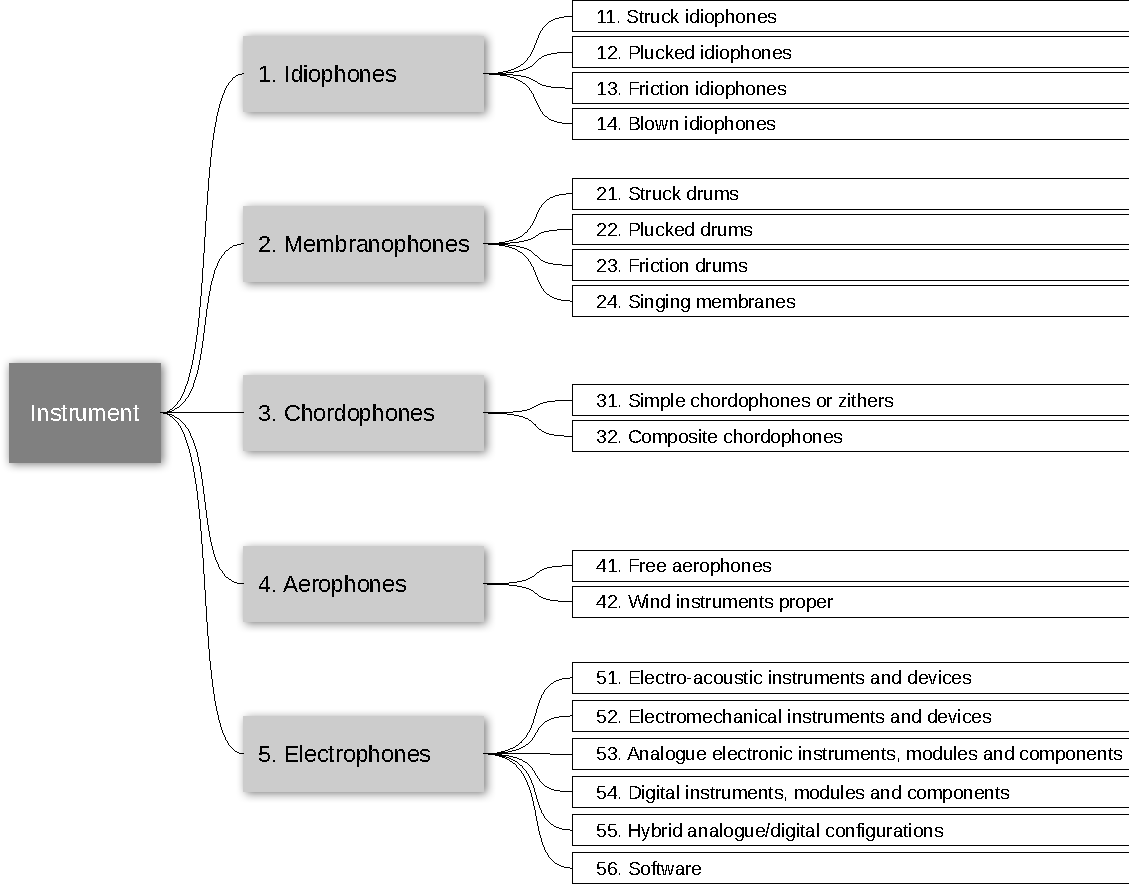
\includegraphics[width=\textwidth]{figures/17-hornbostel-sachs-crop.pdf}
			\caption{The two first layers of the updated Hornbostel Sachs system, based on \citep{mimo_revision_2011}.}
			\label{fig:hornbostel}
}
\end{figure}


\section{Other organologies}

Despite its shortcomings, the Hornbostel Sachs system works reasonably well for many traditional instruments. It has met criticism over the years \citep{lee_hornbostel-sachs_2019}, but continues to be the de facto standard used in instrument catalogs and museums. For such usage, its categorical, tree-like structure helps to categorize different instruments.

There have been several attempts at extending the Hornbostel Sachs system over the years. For example, \citet{olsen_is_1986} proposed \emph{corpophones} as a category to describe vibrations produced by body parts. Interestingly, he does not include the voice in this category, arguing that musical vocal sounds are songs.
\emph{Fictophones} is another proposed category describing imaginary instruments. As \citet{loughridge_museum_2013} write in their introduction of the online Museum of Imaginary Musical Instruments:

\begin{quote}
Imaginary instruments are a special kind of technological phenomenon. Such instruments never fully make the passage from the imagination into the world. They remain unconsummated objects, indifferent to the chaotic forces at play outside the test-tube of pure conceptuality. Ranging from the physically impossible to the simply impractical, from the ``never'' to the ``not yet,'' imaginary instruments rattle suggestively at the windowpane separating our comfortable sense of reality from that nebulous space beyond. In the words of Ernst Cassirer, such instruments are ``concerned in the final analysis not with what \emph{is}, but with what \emph{could be}.''
\end{quote}

This way of thinking about imaginary instruments resonates well with my techno-cognitive approach. After all, an imaginary instrument can also lead to musical experiences. Even if there is no external physical representation of any music being played, there are many accounts of vivid experiences based on musical imagination \citep{grimshaw-aagaard_oxford_2019}.

There have also been attempts at developing entirely new organological systems  \citep[see overviews in][]{kvifte_instruments_1989,magnusson_musical_2017}. Of these, I find the physics-based organology by \citet{mann_natural_2007} intriguing because he proposes a matrix in which the instrument's sound-producing element is split from its user interface element. This opens for different types of explorations with new instruments and performance techniques. Indeed, for him, the system has also represented a tool for instrument design and musical exploration. Many of the older classification systems were intended for instrument classification for museums and research. I am more concerned with how instruments are used, and I will therefore base my classification on such a division between sound-production and sound-modification.

In a similar line of thought, \citet{magnusson_musical_2017} suggests that the shared usage of instruments can be considered a pool of possibilities from which the instrument definition can be found. He calls this a `heterarchical approach to digital organology.' The aim is to break away from the traditional tree-like classification systems and instead focus on the instrument's material design and technical origins.

I think all of these alternative instrument definitions have their pros and cons. They help to broaden and challenge our thinking about musical instruments. However, a challenge with the more open-ended instrument definitions is that they risk being so `fuzzy' that they are challenging to use in practice. My aim is not to create a system that covers everything. Instead, I want to create a theoretical framework to understand what an instrument is, how it is used, and how it is perceived. This includes understanding more about the differences (and similarities) between acoustic and electro-acoustic instruments.


\section{Embodied organology}\label{sec:voice}

The voice has traditionally been left out of organological classifications. This is not strange if one thinks about instruments as physical objects that can be put on a shelf in a museum. However, the voice should be included if one thinks of an instrument as a vehicle for musical expression.

\citet{kreiman_foundations_2011} describe the voice as a \emph{bioacoustical instrument} with a two-stage sound production. The first part is creating a fundamental frequency and related harmonics, which are the basis for the perceived pitch of the vocal sound. The second part is shaping the timbral qualities of the sound through formant frequencies that are resonances of the vocal tract. As such, the voice comprises both sound-producing and sound-modifying parts as any other acoustical instrument. The main difference is that all of the parts are literally embodied within the performer.

The lack of inclusion of the voice in traditional organology also has a cultural dimension. Discussing the changing voice of Maria Callas after her weight-loss, \citet[p.16]{eidsheim_maria_2017} argues for a critical vocal organology:

\begin{quotation}
Investigating the body, which is burdened by millennia of social practices, is one small step in the process of unsticking the female (and the raced, classed and so on) body and voice from their construction and existence within a social and cultural sphere that can only comprehend them from within its own set of resources and hierarchies. In my assessment, critical vocal organology does so not by avoiding, but by addressing head-on, the sociocultural material dimensions of voice.
\end{quotation}

Several others have also called for thinking more about the body when describing instruments. \citet[p.48]{kvifte_what_2008} criticizes instrument definitions that leave out the human body, commenting that in traditional organology, `the instrument is what is left behind when the performer is no longer present.' He exemplifies this with the \emph{trump} (also known as Jew's harp, guimbarde, and maultrommel), an instrument that consists of a flexible reed attached to a frame (Figure~\ref{fig:munnharpe}). This is an instrument that relies on the performer's mouth cavity for sound production and modification. What is then part of the instrument? The mouth of the performer, the lungs, the entire body?
If one agrees that the body is part of a trump, what about other instruments with a physical connection between a performer and the instrument? For example, the fingers of a violin player touch the strings and are also essential for music-making. Should they, too, be considered part of the instrument?
Instead, one may classify instruments after how they are performed. \citet{kvifte_instruments_1989} builds on the model by  \citet{heyde_grundlagen_1975}, separating between \emph{technopomorphic} and \emph{anthropomorphic} elements of instruments. That is, an instrument's function can be split into mechanical and human elements, respectively. Then it is also possible to more directly analyze the interaction between body parts and controllers on the instrument.

\begin{figure}[tbp]
	\centerline{
      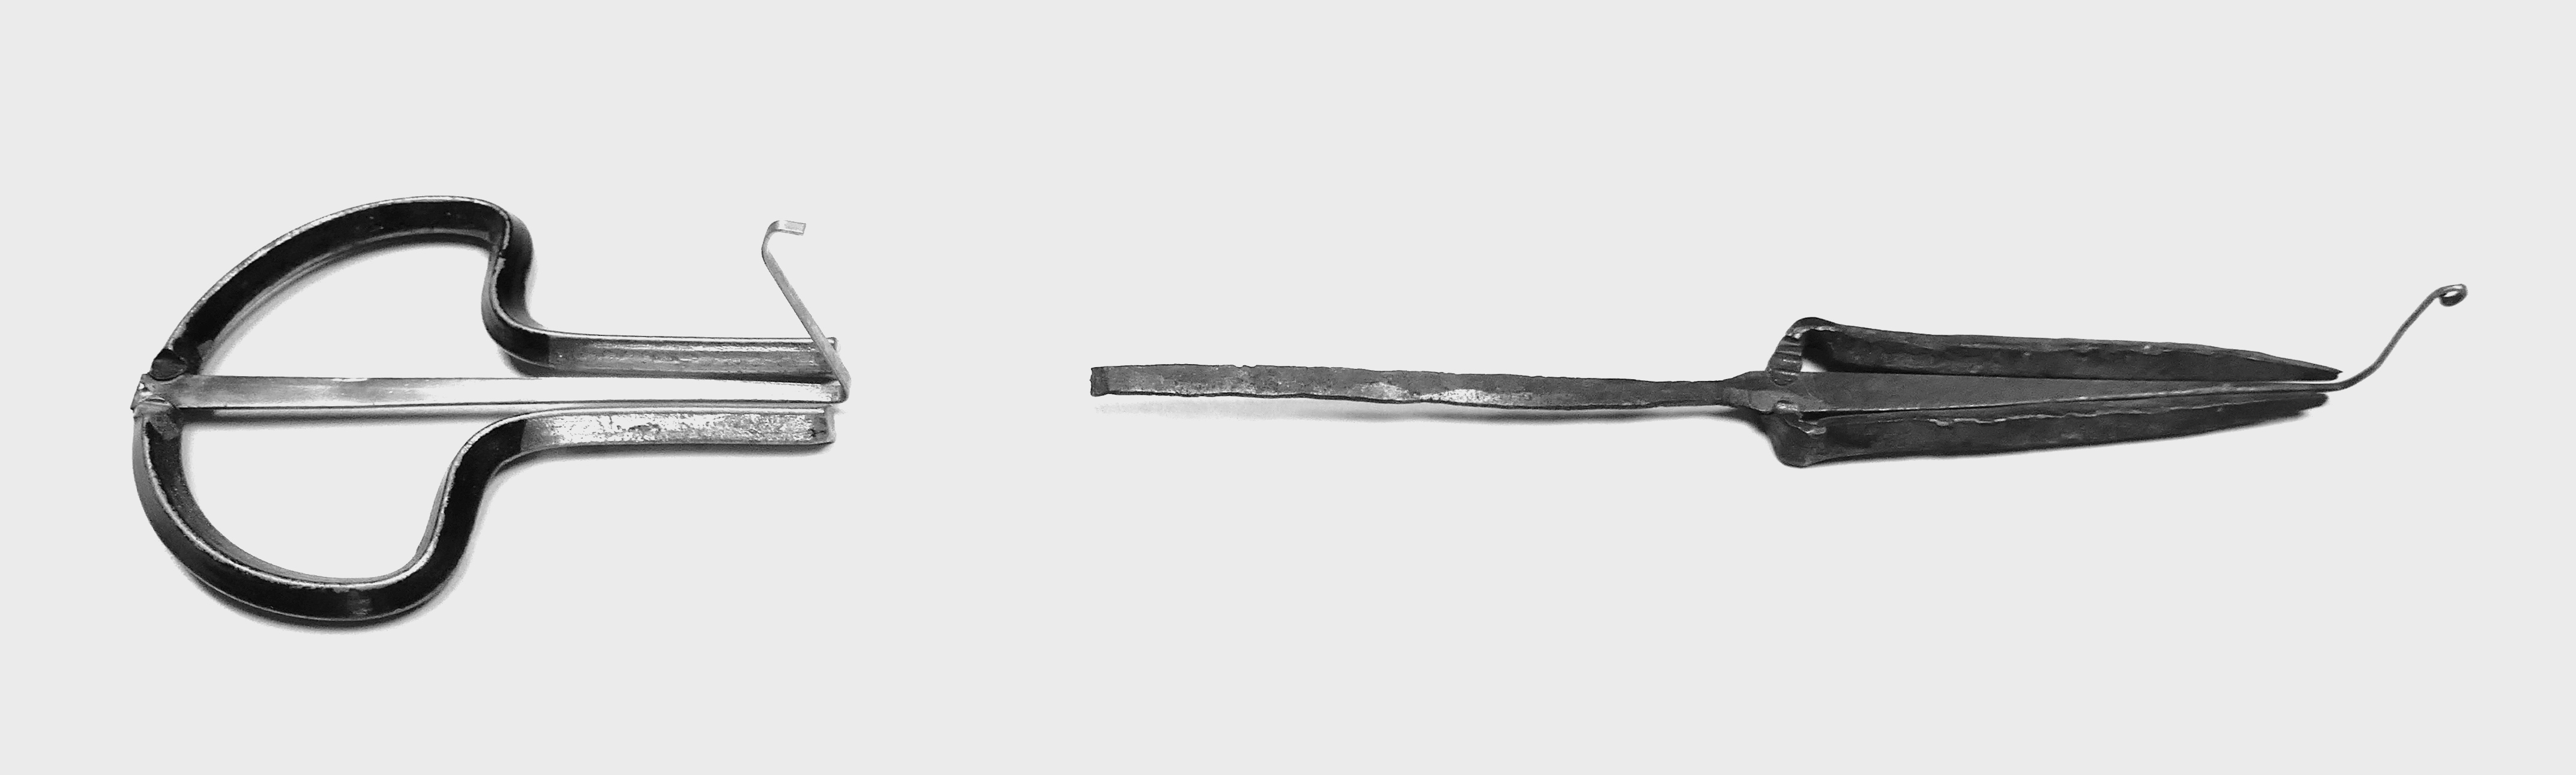
\includegraphics[width=\textwidth]{figures/18-trumps.jpg}
      \caption{Examples of a modern trump (left) and a replica of an old one (right). These instruments require the cavity of the mouth for sound production.}
      \label{fig:munnharpe}}
\end{figure}

A similar line of thought is present in the writings of \citet{paine_interaction_2015} on the \emph{techno-somatic dimension}. Paine sees this dimension as a meeting point between the physical instrument itself and how the human acts upon that instrument. This techno-somatic dimension contains two parts. The technical relates to instrumental technique and performance practice, while the somatic concerns the bodily experience. This resonates with the techno-cognitive approach I propose in my action--sound theory.


\section{Ethno-organology}

\citet{magnusson_migration_2021} argues for an \emph{ethno-organology} that takes into account how instruments move between cultures. He argues that technology is never independent of societies. Instruments are developed within one culture, but they are also used in others. How does such `instrument migration' affect others?

\citet{ahrens_technological_1996} discuss the development of wind instruments during the 19th century. Instrument makers started equipping woodwinds with a linked key mechanism and brass instruments with valves. These technical developments improved the intonation, facilitated playing, and increased the pitch range of the instruments. However, these improvements came at the cost of a larger action--sound separation. On a silver flute, the fingers are no longer in direct control with the sound hole. A vibrato can no longer be created by simple moving the fingers over the sound holes. Instead, a vibrato needs to be produced by the lips. Many such modifications changed the way instruments are played. In addition, we have seen a standardization to follow twelve-tone equal temperament.

The professionalization of instrument makers and uniformation of instrument types have led to the standardization of today's Western traditional instruments. It may be easy to forget that these instruments have been been through numerous development iterations. There is---and has always been---a lot of experimentation with musical instrument designs. This experimentation is culturally dependent. \citet[p.177]{magnusson_migration_2021} cautions against thinking about universality:

\begin{quotation}
	[\ldots] music is \emph{not} a universal language: music changes over time, it travels and adapts to cultural contexts, and it is deeply rooted in instruments and other musical technologies. All over the world, there are house-holds whose family members do not understand each other’s music (for example, a dad not understanding his teenage daughter’s music and vice versa) and very often this rift is caused by the distinct technology used in the production and consumption of the music.
\end{quotation}

Instruments can be seen as a cultural object that can be explored by anyone. New musical ideas are created in the meeting point between an instrument and a performer. \citet{magnusson_ergomimesis_2018} calls this the \emph{ergodynamics} of the instrument, to explain an instrument's expression potential conveyed through its possibilities and limitations. Each performer will bring their own musical and cultural background into the exploration of a new instrument. The result will again influence others. An ethno-organological approach is based on understanding the culture an instrument comes from, how it moves geographically, and how it is used in various other cultures. This involves both historical and techno-cultural investigations.

In a similar line of thought, \citet{morreale_where_2021} calls for reflection on the neo-colonialist tendency of contemporary music technologies. While his discussion is focused on the use of artifical intelligence in music creation, the same can be said about the way digital music technologies spread around the world. For example, most electro-acoustic instruments and digital audio workstations are currently based on twelve-tone equal temperament and grid-based metric structures. This means that they are incompatible with music cultures that rely on microtonal or microrhythmic structures. It is critical that we are aware of the cultural implications of technological developments. Making more flexible music technologies is one way of allowing for more musical diversity.
